
%%%%%%%%%%%%%%%%%%%%%%%%%%%%%%%%%%%%%%%%%%%%%%%%%%%%%%%%%%%%%%%%%%%%%
%% This is a (brief) model paper using the achemso class
%% The document class accepts keyval options, which should include
%% the target journal and optionally the manuscript type.
%%%%%%%%%%%%%%%%%%%%%%%%%%%%%%%%%%%%%%%%%%%%%%%%%%%%%%%%%%%%%%%%%%%%%
\documentclass[journal=jcdis8,manuscript=article]{achemso}

%%%%%%%%%%%%%%%%%%%%%%%%%%%%%%%%%%%%%%%%%%%%%%%%%%%%%%%%%%%%%%%%%%%%%
%% Place any additional packages needed here.  Only include packages
%% which are essential, to avoid problems later.
%%%%%%%%%%%%%%%%%%%%%%%%%%%%%%%%%%%%%%%%%%%%%%%%%%%%%%%%%%%%%%%%%%%%%
\usepackage{chemformula} % Formula subscripts using \ch{}
\usepackage[T1]{fontenc} % Use modern font encodings

%%%%%%%%%%%%%%%%%%%%%%%%%%%%%%%%%%%%%%%%%%%%%%%%%%%%%%%%%%%%%%%%%%%%%
%% If issues arise when submitting your manuscript, you may want to
%% un-comment the next line.  This provides information on the
%% version of every file you have used.
%%%%%%%%%%%%%%%%%%%%%%%%%%%%%%%%%%%%%%%%%%%%%%%%%%%%%%%%%%%%%%%%%%%%%
%%\listfiles

%%%%%%%%%%%%%%%%%%%%%%%%%%%%%%%%%%%%%%%%%%%%%%%%%%%%%%%%%%%%%%%%%%%%%
%% Place any additional macros here.  Please use \newcommand* where
%% possible, and avoid layout-changing macros (which are not used
%% when typesetting).
%%%%%%%%%%%%%%%%%%%%%%%%%%%%%%%%%%%%%%%%%%%%%%%%%%%%%%%%%%%%%%%%%%%%%
\newcommand*\mycommand[1]{\texttt{\emph{#1}}}

%%%%%%%%%%%%%%%%%%%%%%%%%%%%%%%%%%%%%%%%%%%%%%%%%%%%%%%%%%%%%%%%%%%%%
%% Meta-data block
%% ---------------
%% Each author should be given as a separate \author command.
%%
%% Corresponding authors should have an e-mail given after the author
%% name as an \email command. Phone and fax numbers can be given
%% using \phone and \fax, respectively; this information is optional.
%%
%% The affiliation of authors is given after the authors; each
%% \affiliation command applies to all preceding authors not already
%% assigned an affiliation.
%%
%% The affiliation takes an option argument for the short name.  This
%% will typically be something like "University of Somewhere".
%%
%% The \altaffiliation macro should be used for new address, etc.
%% On the other hand, \alsoaffiliation is used on a per author basis
%% when authors are associated with multiple institutions.
%%%%%%%%%%%%%%%%%%%%%%%%%%%%%%%%%%%%%%%%%%%%%%%%%%%%%%%%%%%%%%%%%%%%%

\author{Wenxi Zhao}
\author{Dmitriy Korobskiy}
\author{Shreya Chandrasekharan}
\affiliation[NET ESolutions Corporation (an NTT DATA Company)]{Netelabs, NET ESolutions Corporation, VA, USA}
\author{Kenneth Merz}
\email{merz@msu.edu}
\affiliation[Michigan State University]{Department of Chemistry, Michigan State University, MI, USA}

\author{George Chacko}
\email{chackoge@illinois.edu}
\affiliation[University of Illinois Urbana-Champaign]{Dept. of Computer Science, University of Illinois Urbana-Champaign, IL, USA}
\alsoaffiliation[University of Illinois Urbana-Champaign]{Grainger College of Engineering, University of Illinois Urbana-Champaign, IL, USA}
\altaffiliation{Previous address: Netelabs, NET ESolutions Corporation, VA, USA}


\title{Converging Interests- Chemoinformatics, History, and Bibliometrics}
%\date{}							% Activate to display a given date or no date

\begin{document}
%maketitle
%\section{}
%\subsection{}

\begin{tocentry}
Some journals require a graphical entry for the Table of Contents.
This should be laid out ``print ready'' so that the sizing of the
text is correct.

Inside the \texttt{tocentry} environment, the font used is Helvetica
8\,pt, as required by \emph{Journal of the American Chemical
Society}.

The surrounding frame is 9\,cm by 3.5\,cm, which is the maximum
permitted for  \emph{Journal of the American Chemical Society}
graphical table of content entries. The box will not resize if the
content is too big: instead it will overflow the edge of the box.

This box and the associated title will always be printed on a
separate page at the end of the document.

\end{tocentry}

\begin{abstract}

Modern scientometric techniques, applied at scale, can provide valuable information that complements qualitative investigation of the accumulation of knowledge in a field. We discuss a trio of articles from computational chemistry selected from an analysis of 181 million tri-cited 
articles. 

\end{abstract}

\section{Viewpoint}

The chemoinformatics literature has been analyzed by Willett~\citep{willett2008}, who noted that  `Chemoinformatics first appeared as a distinct discipline in the late-Nineties, since when it has generated a considerable literature'. Willett cites preceding work by Onodera~\citep{onodera2003} on chemical informatics, and also references methods from scientometrics. Of these, algorithmic historiography~\citep{garfield2004} merits special mention since it involves constructing a historical record using scientific citations. The chemoinformatics community has thus experienced intersections with science history and bibliometrics (the terms bibliometrics and scientometrics are often interchangeably used). 

Williams and colleagues (2015)\citep{williams2015scientific} used the principles of algorithmic historiography coupled with data mining and network analysis to describe two very large collaboration networks that contributed to the basic and translational work preceding the development of breakthrough drugs. We have extended this work to analyze, on a greater scale, similar networks for five anti-cancer drugs also approved for human use by the Food and Drug Administration (FDA), a study that involved analyzing the work of 235,000 authors of 106,000 publications. 

Modern bibliographic databases such as Scopus and Web of Science greatly assist such studies since their coverage is extensive; their content (available through a commercial license) can be incorporated into relational or graph databases for large scale analysis. Citation data are neither complete nor error free but are still immensely useful, and the data available today are improved over what was available decades ago. We emphasize that citations can tell only a part of a story but are valuable in tracing developments in a field, and the consideration of new ideas within it.  

In this Viewpoint, we use the quantum mechanical (QM) density functional theory (DFT) model referred to as B3LYP as a case study. B3 refers to the Becke 3-parameter Exchange functional and LYP to the Lee, Yang and Parr Correlation functional.

Three major patterns of citation have been described: (i) direct citation (ii) bibliographic coupling and (iii) co-citation. When an article cites or references another article a direct citation link is created between the citing article and its target, the cited article. Many such links to a cited article causes it to accumulate citations, which are sometimes used to estimate its impact. When two articles cite a third, they are bibliographically coupled. When two articles are cited by a third, they are said to be co-cited with the implication that two previously existing ideas are combined into a new one. 

Co-citation, the third, was independently described by Irina Marshakova-Shaikevich and Henry Small in 1973~\citep{MarshakovaShaikevich1973,Small1973} and co-citation measurements have since been extensively used in scientometrics. The frequency of co-citation of a pair of articles  also accumulates over time and represents the extent to which this new idea is recognized by the research community. In this respect, co-citation is a dynamic measure compared to bibliographic coupling. The vast majority of articles are cited or co-cited once or not at all so highly cited or co-cited articles naturally pique interest. 

In 1973, Henry Small reported 4 pairs of articles with a co-citation frequency of 49 and greater from a sampling of the physics literature. The volume of scientific literature has since grown considerably; more co-cited pairs have been discovered, citation frequencies have increased, and the scale of bibliometric studies has also increased. Improved bibliographies and modern computing tools have also rendered co-citation calculations relatively facile and co-citation has been measured over tens of millions of articles, and the high end of co-citation frequencies is in the tens of thousands. Interestingly, in a large scale study of co-citation patterns across the all scientific literature, the articles by (i) Becke (1993)\citep{becke1993dft} and (ii) Lee, Yang, and Parr (1988)\citep{lyp1988} were the most highly co-cited pair of 33 million such pairs that we studied. 

A natural extension of co-citation theory is document coupling of a higher order, for example, triads and tetrads that are correspondingly tri-cited and tetra-cited. It is possible to view any article $A$ that cites $n$ articles as comprising $n$ citations, $n\choose2$ co-citations, $n\choose3$ tri-citations and so on. Indeed, Henry Small, in 1974,  proposed a model of multiple citation based on tri-citations measured over a set of 6 publications.  Calculating the frequencies of these combinations in a bibliography is relatively expensive, however, and may have dissuaded follow-up investigations. For example, an article with either 25 or 50 cited references represents 300 or 1,225 co-citations respectively. The same article also consists of  2,300 or 19,600 tri-citations and  12,650 or  230,300 tetra-citations. For even a modestly sized collection of 2 million articles with an average of 30 references each, this could involve computing $8.12\times10^9$ tri-citations, $5.48\times10^{10}$ tetra-citations, or $2.85\times10^{11}$ penta-citations. However, today's computing resources place documenting these higher order structures within reach of the scientometrist, and opens a frontier for discovery that extends beyond co-citation.

In an initial exploration of higher-order combinations, we have used a `brute force' approach to compute the tri-citation frequencies of 181 million triads from 11 years of articles in the Scopus bibliography.  Much like citations and co-citations, the vast majority of tri-citations are of very low frequency, suggesting modest community recognition. High frequency triplets are therefore, of interest. The triad with the highest frequency that we observed in 181 million cases has been tri-cited at least 13,000 times and all three of its component articles derive from density functional theory (DFT). 
\begin{figure}[h!]
\begin{center}
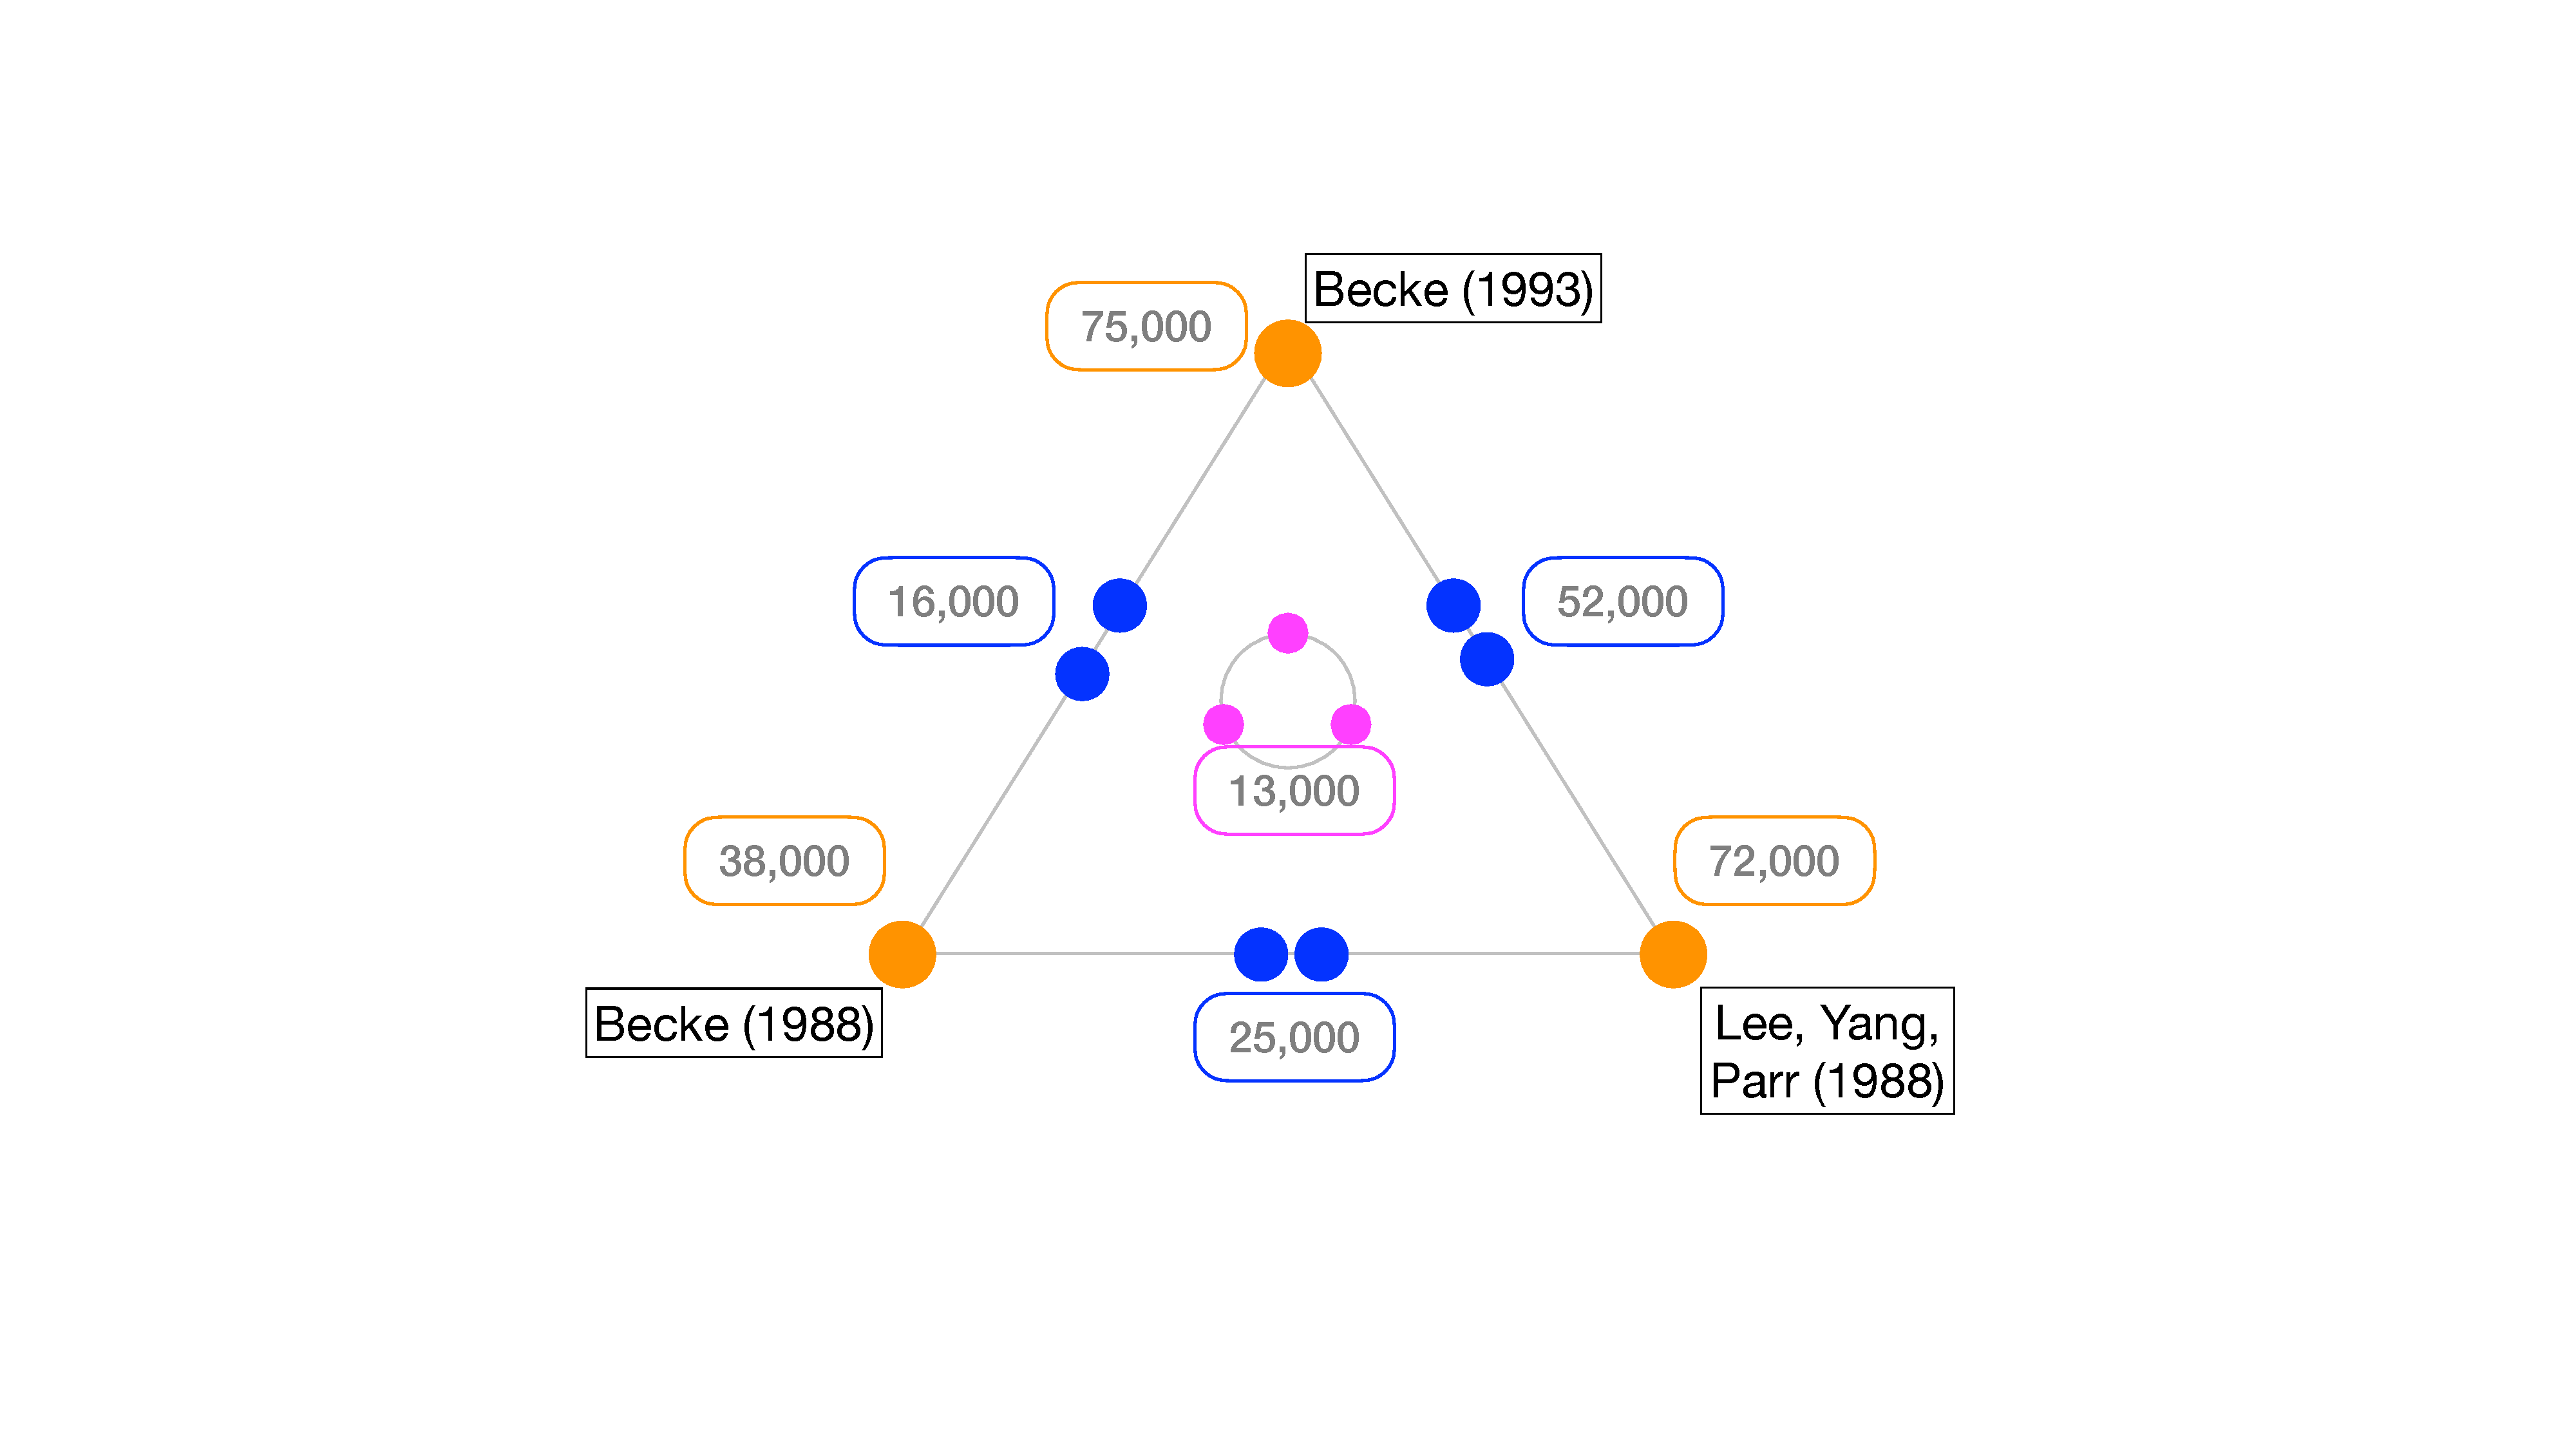
\includegraphics[width=10cm]{fig1_tricite.pdf}% This is a *.eps file
\end{center}
\caption{A high frequency triplet. The triad of (i) Becke (1988), (ii) Becke (1993), and (iii) Lee, Yang, and Parr (1988).  Frequencies (rounded rectangles) are shown for the tri-citation (center of triangle), co-citations (sides of triangle), and article citations (vertices of triangle). All frequencies shown have been rounded down to the nearest thousand
}
\label{fig:fig1}
\end{figure}

The origin of this triad appears to trace back to 1994, when Stephens, Chabalowski, Devlin, and Frisch~\citep{stephens1994ab} blended the B3 Exchange and LYP Correlation functionals into a hybrid functional method currently  referred to as B3LYP.  In the B3LYP model, two functionals of the electron density are needed. One is the Exchange functional (two electrons of the same spin cannot be at the same point in space) and the other is the Correlation functional (accounting for the correlated motion of electrons with the same spin). The first referencing of this triad appears to be in two reports in 1993: an article by Laming, Temath, and Handy\citep{laming1993} titled `A general purpose exchange‐correlation energy functional', and a chapter titled `Theoretical Organic Chemistry' in Annual Reports Section ``B" (Organic Chemistry) by Reynolds\citep{reynolds1993theoretical}.

The B3LYP method had a lot of advantages in terms of speed and accuracy, especially for the study of organic molecules, and was rapidly adopted by the computational chemistry and organic chemistry communities. Historically, B3LYP originates from an effort in the 1980s to to build Exchange and Correlation functionals to allow for the practical application of DFT to chemical problems. A number of research groups engaged and the Becke group in 1988 and 1993 described a hybrid functional~\citep{becke1988density}, and an Exchange functional~\citep{becke1993dft}, respectively, while Lee, Yang, and Parr (LYP) developed a Correlation functional in their 1988 paper~\citep{lyp1988}.  

This major advance can be concisely referenced by citing Becke-1988~\citep{becke1988density}, LYP-1988~\citep{lyp1988} and Becke-1993~\citep{becke1993dft} since the two Becke articles represent the Exchange functional and the Lee-Yang-Parr article contributes the Correlation functional. The high frequency of co-citation (52,000) of Becke-1993 and LYP-1988 may result from authors assuming or concluding that citing Becke's 1993 article is adequate to reference the Exchange functional. 

Based on our use of Scopus data, the three articles in the Becke-1988--LYP-1988--Becke-1993 triad appear to have been co-cited at least 16,000, 25,000, and 52,000 times respectively, and the individual articles cited at least 38,000, 72,000, and 75,000 times (Figure 1). It is more difficult to conjecture why these three articles are individually cited at these very high levels although it is worth noting that  frequencies of article citations always exceed those of co-citations, which in turn exceed those of tri-citations. It is also very likely that these articles have individually stimulated new ideas.

An interesting community discussion thread~\citep{johansson2002} provides the opinion that a complete set of citations for B3LYP is (i) Vosko, Wilk and Nusair, 1980~\citep{vosko1980accurate} or VWN-1980 (ii) Becke-1988 (iii) LYP-1988) (iv) Becke-1993 and (v) Stephens, Chabalowski, Devlin, and Frisch (1994) or SCDF-1994. It is interesting to note that VWN-1980  is not apparently cited in Becke (1988), Becke (1993), or LYP (1993) although it is cited in Laming et al. (1993), Reynolds (1993), and SCDF-1994.

In summary, we describe a high frequency triad discovered through a discipline-agnostic search that led us to a cluster of publications that are associated with a major advance in  in the practical application of DFT to chemical and biological problems. Examining the three component co-cited pairs of the triad allows us to infer that Becke (1993) and LYP (1988) are most extensively recognized in the community as far as B3LYP is concerned. Why Becke-1988 is not more often co-cited with Becke (1993) and LYP (1988) is an interesting question along with why VWN (1980) is not generally included with these three papers forming a highly cited cluster of four papers. The same question can be asked regarding SCDF (1994) which merged the technologies of these these four publications into what is now known as the B3LYP Exchange-Correlation function.  Inferring or understanding the social behavior in the community that resulted in these citation patterns will require further qualitative research. In the meantime, it may be reasonable to conclude that B3LYP has had high impact in computational chemistry and and generates curiosity in the chemoinformatics  and scientometrics worlds.

%\bibliographystyle{acm}
\bibliography{B3LYP}

\end{document}  